\documentclass{article}
\usepackage[utf8]{inputenc}
\usepackage{graphicx}
\usepackage{float}
\usepackage{listings}
\usepackage{hyperref}
\usepackage{amsmath}
\usepackage{commath}
\usepackage{tabularx}
\usepackage[ruled,vlined]{algorithm2e}
\graphicspath{{./plots/}}
\usepackage{biblatex}
\addbibresource{referanse4.bib}
\usepackage{caption}
\usepackage{subcaption}


\hypersetup{
    colorlinks=true,
    linkcolor=blue
}

\title{\textbf{Phase transition simulation using the Ising model and Monte Carlo methods} \\ FYS3150 - Project 4}
\author{Authored by Philip Hoel, Theo G. Halvorsen \\ and Elakkyen Pathmanathan}
\date{\today}

\begin{document}

\maketitle

\begin{figure}
    \includegraphics[scale=0.6]{Project1/UiO.jpg}
\end{figure}

\newpage

\tableofcontents
\newpage

\section{Abstract}
We simulate the phase transition of an arbitrary ferromagnetic material using the well known ising model in two dimensions. Finding the critical point of the material. We will present a quick look at the analytical model and how it works, before we go in depth in how the numerical model works. By using a Monte Carlo method, we increase the efficiency of the ising model. The Monte Carlo method we use and will be more familiar with is the metropolis algorithm.

\section{Introduction}

In this project, we will simulate phase transitions of magnetization in an arbitrary ferromagnetic material. This phase transition will go between magnetized and not magnetized and will be referred to as spin. To simulate, we will use a widely known model, called the Ising model. The Ising model is binary and thus is perfect for our binary system. It has many uses and has, for example, been used to model the United States of America's presidential election. Since we are looking at systems with a large degree of freedom, the system's total number of possible states becomes enormous. That means we have to limit ourselves to specific conditions, which naturally brings some problems. That leads us to statistical physics methods with the Monte Carlo based Metropolis algorithm.  Before taking on the phase transition simulation, we make sure to use the correct data by approximate the system's most likely energy state. With the mentioned method, we can obtain a system's most likely state without calculating every possibility.
\newline
\newline
We will start off by explaining the methods of use from statistical mechanics, such as the Monte Carlo method and the metropolis algorithm, eventually defining the Ising model. After that, we will talk about the implementation and discuss the results.

\newpage
\section{Theory}

Statistical physics is a field that builds a link between microscopic events and macroscopic properties in a physical system. Macroscopic properties are then, for example, heat and pressure.  Statistical physics addresses all possible states for a system to be in on a microscopic level. This is called an ensemble, a collection of possible conditions for a system to be in. This collection gives us a probability distribution for the system, where we can extract and associate different system properties. There are different kinds of ensembles, depending on the purpose.  We will be focusing on the thermodynamic ensembles, or so-called equilibrium ensembles, which describe an isolated system under temperature equilibrium where the different states are at different energy levels, and the probabilities are distributed accordingly. \newline
This gives macroscopic relationships to classical thermodynamics based on probability theory and physic laws. Intuitively it allows us to extract information from a system with infinitely many particles by just looking at the microscopic constituents' fundamental interactions between particles.  As mentioned, the ensembles give us a probability function in which we can obtain different properties. The probability for a given state is provided by the Probability Distribution Function(PDF).

\begin{equation}
    P(E_{i}) = \frac{e^{-E_i\beta}}{Z}
\end{equation}
Where $i$ is the state, $E_i$ is the state's total energy, $\beta=\frac{1}{k_BT}$, $k_B$ is the Boltzmann's constant, $T$ is the temperature, and $Z$ is the partition function.

\noindent The partition function sums over all possible microstates and works like a normalization constant. It is defined as
\begin{equation}
    Z=\sum_{i}^{N}e^{-\beta E_i}
\end{equation}
With the probability function (1), we can further calculate different states and then find the system's expectation value of the energy E and the magnetization M. The expected value is an average of all the possible outcomes. If all outcomes are equiprobable, this becomes the simple arithmetic mean, which is the sum of all values divided by the number of outcomes, which is the partition function. With the use of the PDF, we get 
%%% kilde er STK1100 boken side 112%%%
\begin{equation}
    \langle E\rangle = \sum_{i}^NE_{i}P(E_{i}) = \frac{1}{Z}\sum_{i}^NE_{i}e^{-\beta E_{i}}
\end{equation}
\begin{equation}
   \langle \abs{M} \rangle = \sum_{i}^N\abs{M_{i}}P(E_{i}) = \frac{1}{Z}\sum_{i}^NM_{i}e^{-\beta E_{i}}
\end{equation}
\newline \newline

%%% Kilde STK1100 boken siden 117 %%%
Another useful property of the field of statistics is variance. The variance is a measure of the variability in the distribution of a random variable X. The variance is defined as
$$V(X) = \sum_{x \in D}(x - \mu)^2 \cdot p(x)$$
here $D$ is the set of outcomes, $p(x)$ is the pdf and $\mu$ is the expected variable. If we now change around on the equation.
\begin{align}
    V(X) & = \langle (x - \mu)^2 \rangle \\
    V(X) & = \langle (x^2 - 2x \mu + \mu^2)\rangle \\
    V(X) & = \langle x^2 \rangle - 2\langle x \rangle \mu + \mu^2 \\
    V(X) & = \langle x^2 \rangle - 2 \langle x \rangle \langle x \rangle + \langle x \rangle^2 \\
    V(X) & = \langle x^2 \rangle - \langle x \rangle^2
\end{align}
The variance can also be written $\sigma^{2}_{X}$. When we replace X with E and M, we thus get the energy and magnetization variance
$$\sigma_{E}^{2} = \langle E^2 \rangle - \langle E \rangle^2$$
$$\sigma_{M}^{2} = \langle \abs{M}^2 \rangle - \langle \abs{M} \rangle^2$$
%\paragraph{Correlation Function}
From the functions above we can derive both the specific heat constant and the susceptibility.
$$C_{V} = \frac{1}{k_{B}T^2}(\langle E^2 \rangle - \langle E \rangle^2)$$
$$\chi = \frac{1}{k_{B}T}\langle \abs{M}^2 \rangle - \langle \abs{M} \rangle^2$$
The heat constant defines the amount of heat needed to change the temperature by a unit for a material.
The susceptibility calculates how much the material will be magnetized if placed in a magnetic field.
\newline

\noindent When we talk about equilibrium, we are really talking about Helmholtz's free energy. The Helmholtz free energy is a thermodynamic potential in a closed systems. It relates the expected value $\langle E \rangle$ to the entropy $S$. The potential energy of a system is defined as
$$F=\langle E\rangle-TS$$
where $F$ is the Helmholtz free energy. The Helmholtz equation shows the struggle between energy and entropy in the system. These two properties competes to achieve minimum energy and maximal entropy. At Thermal equilibrium these two properties will be in balance at a given temperature thereby reducing the Helmholtz free energy.
\subsection{Phase Transitions}
Phase transition is defined as change of property from outer factors such as temperature and pressure. At  the critical point a transition will occur, in our case loss of magnetization. This means it is possible to define the change of mean magnetization up to this critical point(critical temperature $T_c$)
$$\langle \abs{M} \rangle\sim(T-T_c)^\beta$$
Where $\beta = 1/8$ is a critical exponent. As before we can derive the heat capacity and and the susceptibility.
\newline
\newline The heat capacity
$$C_V(T)\sim(T-T_c)^{-\alpha}$$
The susceptibility
$$\chi(T)\sim(T-T_c)^{-\gamma}$$
with $\alpha = 0$ and $\gamma = -7/4$.
\newline
\newline
The type of phase transition we are looking at is called second-order phase transition. When the correlation length $\xi$ becomes infinitely large at critical temperature. The phases on either side of the critical temperature is identical. The correlation length is given by
$$\xi(T)\sim |T_c-T|^{-\upsilon}$$
Since we are using Ising model in two dimensions our calculations will be on a finite lattice thereby the correlation length will be proportional with the size of the lattice.  We can then use finite size scaling relations to mimic the behavior at finite lattice like if it was a infinitely large lattice. The properties are then proportional to the lattice size $L$ and are defined as
\newline \newline
\paragraph{Critical temperature} where $a$ is a constant.
$$T_c(L)-T_c(L=\infty)\propto aL^{-1/\upsilon}$$
\paragraph{Mean magnetisation}
$$\langle \abs{M} \rangle\propto L^{-\beta/\upsilon}$$
\paragraph{Heat capacity}
$$C_V(T)\propto L^{\alpha/\upsilon}$$
\paragraph{Susceptibility}
$$\chi(T)\propto L^{\gamma/\upsilon}$$
\newline
\newline
With the relations set, we can begin to explain our model.
 
\newpage
\subsection{Ising Model}
%%%%% Check resources %%%%
The Ising model is a mathematical model for modeling ferromagnetic material but has been used in other areas of science. The ising model is a binary model simulating a lattice grid of objects with binary values. In our case, this grid is a grid of particles, with a spin up or a spin down, representing magnetization or not.


\subsubsection{Analytical Model} \label{anal}
We start by solving an analytical model of the Ising model. This is good to be able to further check whether the approaches we take are correct. We create a grid of $2 \times 2$ with the following different configurations
\[
\begin{matrix}
\uparrow & \uparrow \\
\uparrow & \uparrow
\end{matrix}
\qquad
\begin{matrix}
\uparrow & \uparrow \\
\uparrow & \downarrow
\end{matrix}
\qquad
\begin{matrix}
\uparrow & \uparrow \\
\downarrow & \downarrow
\end{matrix}
\qquad
\begin{matrix}
\downarrow & \uparrow \\
\uparrow & \downarrow
\end{matrix}
\]
In the table \ref{tab:my_label} below, we can see the different values of the different configurations. Here we have used the periodic boundary condition. To explain the periodic boundary condition, we use an example. We look at the top row of the table. We have 4 spin ups in this configuration.
\[
\begin{matrix}
\uparrow & \uparrow \\
\uparrow & \uparrow
\end{matrix}
\]
If we now focus on the particle in the top left corner, we add dots for the periodic boundary conditions
\[
\begin{matrix}
 & \cdot & \cdot \\
\cdot & \uparrow & \uparrow \\
\cdot & \uparrow & \uparrow  \\
 & \cdot & \cdot
\end{matrix}
\]
The dot to the left of the focus arrow, mimics the arrow to the right of the focus arrow. For the dot above our focus arrow, it will be the same as the arrow below the focus arrow.
\begin{table}[H]
    \centering
    \begin{tabular}{|c|c|c|c|}
        \hline
        \uparrow & E & \abs{M} & N \\
        \hline
        4 & -8J & 4 & 1 \\
        3 & 0 & 2 & 4 \\
        2_{D} & 8J & 0 & 2 \\
        2 & 0 & 0 & 4 \\
        1 & 0 & 2 & 4 \\
        0 & -8J & 4 & 1 \\
        \hline
    \end{tabular}
    \caption{Values of the different configurations of a $2\times2$ lattice grid. Here $\uparrow$ is the number of particles with spin up, E is the energy, M is magnetization and N is the number of ways to configure that spin-up number.}
    \label{tab:my_label}
\end{table}
\noindent
To find the partition function for a $2 \times 2$ grid, we can use the values in Table 1. For each row 
$$Z =\sum_i N_i \cdot e^{-\beta E_i}$$
This gives us, for our case
$$Z = 4 \cdot cosh(8J\beta) + 12$$
If we now write out all the energy states, we can find an equation for the mean energy.
\begin{equation}
    \begin{split}
    \langle E \rangle & = \frac{1}{Z}\sum_{i}E_ie^{-E_i \beta} \\
     \langle E \rangle & = \frac{-8Je^{8J\beta}}{Z} + \frac{8Je^{-8J\beta}}{Z} + \frac{8Je^{-8J\beta}}{Z} - \frac{-8Je^{8J\beta}}{Z} \\
     \langle E \rangle & = \frac{-32J\cdot sinh(8J\beta)}{Z}
    \end{split}
\end{equation}
If we derive the other equations as well, we get
\begin{equation}
    \begin{split}
        \langle E \rangle & = \frac{-32J\cdot sinh(8J\beta)}{Z} \\
        \langle E^2 \rangle & = \frac{256Jcosh(8J\beta)}{Z} \\
        \langle |M| \rangle & = 8\frac{2 + e^{8J\beta}}{Z} \\
        \langle M^2 \rangle & = 32\frac{1 + e^{8J\beta}}{Z}
    \end{split}
\end{equation}

\newpage
\section{Method}
We are using three different coherent concepts, Monte Carlo simulations, Markov Chains, and the metropolis algorithm. The Monte Carlo simulation is a method of estimating an unknown quantity using inferential statistics principles. The principle of the Monte Carlo simulation is to select random samples of a sample space that forms a representation without including all possibilities. In our case, it is to draw random energy levels. Each energy level is determined by our lattice of spins. This means that we sample random configurations of spins, and all possible combinations of spins are the total sample space, or often called population. \newline
\newline
\noindent
We are interested in the most probable state of the physical system, the thermodynamic equilibrium. To find the most probable state, we can simulate how the physical systems move towards it. 
The path to balance is a sequence of events. We take advantage of this by using the Markov Chain concept. A Markov Chain is a sequence of events where one transition from one event to another is determined by specific probabilistic rules. But we also want to limit ourselves to the "shortest" path to equilibrium, which is the sequence of events that is most likely. The Metropolis algorithm does precisely this. The algorithm starts with a random state, where it calculates mean energy and magnetization. Then it selects a random spin $L^2$ times and calculates the resulting change in energy. We accept the energy and the new modification if the difference in energy is less than zero, else we accept the new state if $e^{-\beta E_i}$ is more significant than a random number r, which are between 0 and 1. We show the algorithm more clearly, step by step, below.     

\subsection{Implementation}
The implementation of the ising model is done using a combination of the programming language C++ and Python. All code can be found at \href{https://github.com/philhoel/Computational-Physics/tree/master/Project4}{Github}, including instructions on how to run the programs.
\newline
\newline
When we have a system with the potential to get an extensive calculation, it is always desirable to optimize. We do this by parallelizing the code and doing some other neat tricks. With parallelization, we make sure to take advantage of each core in the CPU. We do this by dividing the work into subsets and assigning them to each of the cores. The work distribution is done by dividing the number of Monte Carlo cycles to each core, which performs its piece of work, and finally, we collect all the subsets for the finished result. An estimate; our code calculates roughly around
\begin{equation}
    11n^2+24+(25n^2+9)mcs+1
\end{equation}
FLOPs. Where $n$ is the grid size and $mcs$ is Monte Carlo cycles. If we set $n=100$ and $mcs=10^6$, we will get $FLOPs=2.5*10^{10}$, since we have $8$ cores, each core will get roughly $3*10^9$ FLOPs.


\paragraph{Metropolis Algorithm}
\begin{enumerate}
    \item Set $E_b$ to be a random configuration in the lattice
    \item Flip the configuration by one spin. Compute the energy and store as $E_t$
    \item Calculate $\Delta E = E_t - E_b$
    \item If $\Delta E \leq 0$, accept new configuration
    \item If $\Delta E > 0$, calculate $w = e^{-\Delta E \beta}$
    \item Compare $w$ with a random number $r$. If $r \leq w$, accept new configuration, else keep old one
    \item Update various expectation values
    \item Repeat (2) - (7)
    \item Each sweep is a MC cycle. Divide by MC cycles at the end.
\end{enumerate}

\subsubsection{Parallelization}
Even if the metropolis algorithm is and efficient and clever algorithm, with so many Monte Carlo cycles, the algorithm still gets rather computationally heavy. Because of this, we choose to parallelize our code for more efficient runs. We have chosen to use the library called MPI. This let's us run multiple computations on multiple processors at the same time to lower the runtime of the computations of the program.

\newpage
\section{Results}

\begin{figure}[H]
  \begin{subfigure}[b]{0.6\textwidth}
    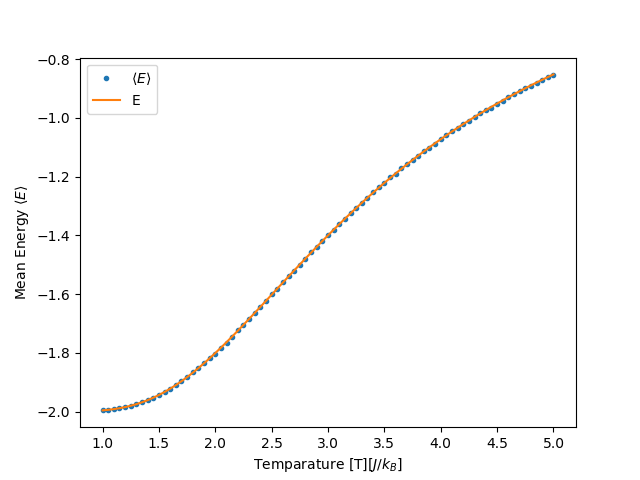
\includegraphics[width=\textwidth]{Project4/plots/average_E_c.png}
    \caption{Mean E}
    \label{fig:meanEA}
  \end{subfigure}
  \hfill
  \begin{subfigure}[b]{0.6\textwidth}
    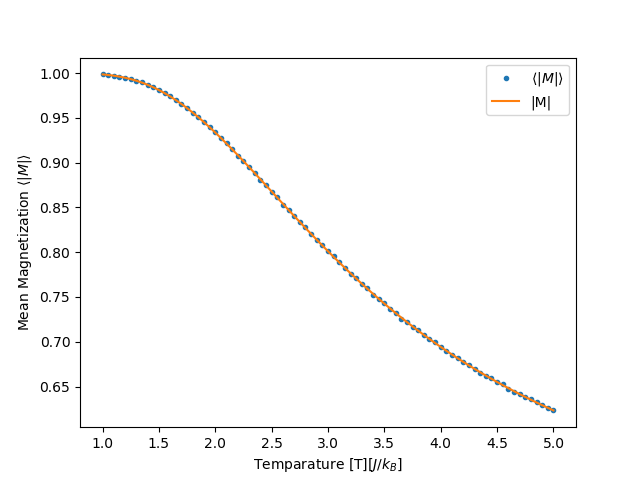
\includegraphics[width=\textwidth]{Project4/plots/average_M_c.png}
    \caption{Mean M}
    \label{fig:meanMA}
  \end{subfigure}
  \caption{The plot shows the analytical and numerical values of the 2x2 lattice grid as a function of temperature. The first plot shows the mean energy and the second shows the mean magnetization}
\end{figure}

\begin{figure}[H]
  \begin{subfigure}[b]{0.6\textwidth}
    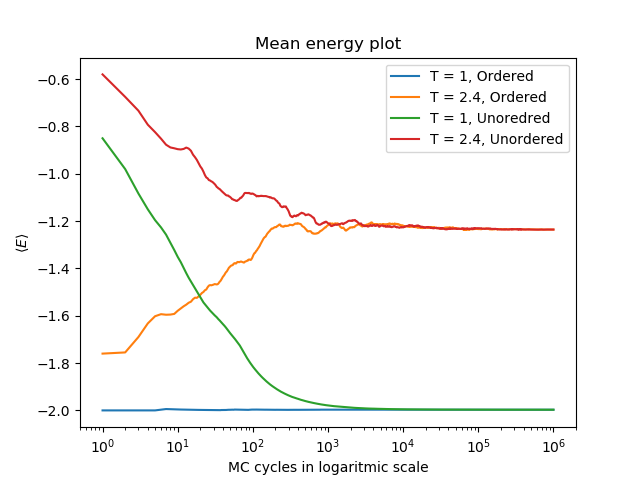
\includegraphics[width=\textwidth]{Project4/plots/problem_d_E.png}
    \caption{Mean E}
    \label{fig:MCE}
  \end{subfigure}
  \hfill
  \begin{subfigure}[b]{0.6\textwidth}
    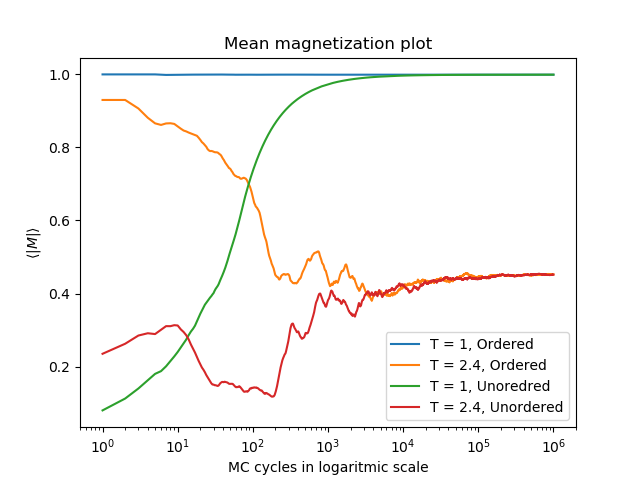
\includegraphics[width=\textwidth]{Project4/plots/problem_d_M.png}
    \caption{Mean M}
    \label{fig:MCM}
  \end{subfigure}
  \caption{Values of the mean energy and mean magnetization as a function of the number of Monte Carlo cycles. The Monte Carlo cycles are in logarithmic scale. The plot show values for initialization of a ordered grid in both temperature $T=1$ and $T=2.4$ and the values for initialization of a unordered grid in the same temperature.}
\end{figure}

\begin{figure}[H]
  \begin{subfigure}[b]{0.6\textwidth}
    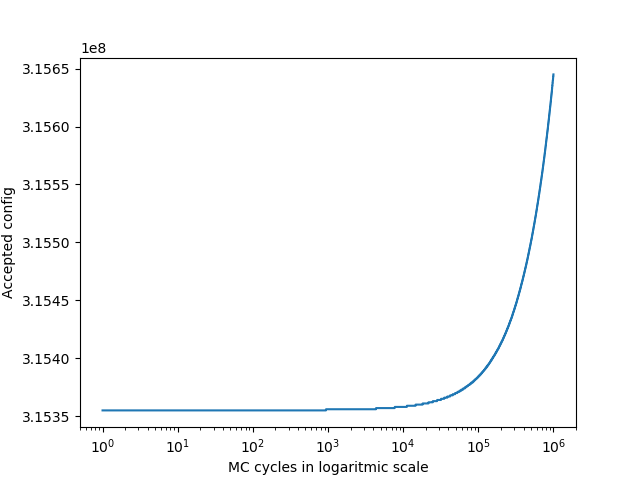
\includegraphics[width=\textwidth]{Project4/plots/Acc_MC.png}
    \caption{Accepted Configurations MC}
    \label{fig:accMC}
  \end{subfigure}
  \hfill
  \begin{subfigure}[b]{0.6\textwidth}
    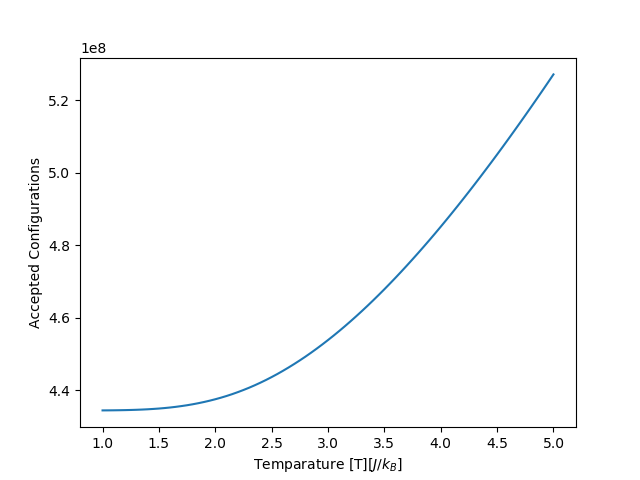
\includegraphics[width=\textwidth]{Project4/plots/Acc_temp.png}
    \caption{Accepted Configurations Temp}
    \label{fig:accTemp}
  \end{subfigure}
  \caption{Showing the number of accepted configurations as a function of both Monte Carlo cycles and temperature}
\end{figure}

\begin{figure}[H]
    \centering
    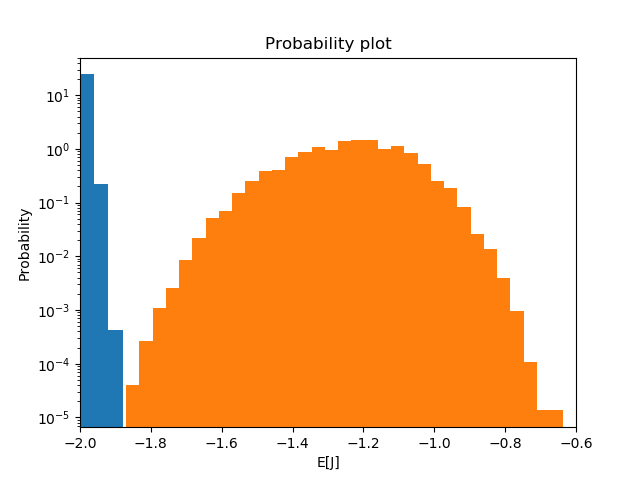
\includegraphics[scale=0.5]{Project4/plots/problem_e.png}
    \caption{The plot shows a histogram of the probability of each energy. The blue values are the probability for $T = 1$ and the orange is the probability for $T = 2.4$. Both systems are grid size $20\times 20$.}
    \label{fig:prob}
\end{figure}

\begin{figure}[H]
  \begin{subfigure}[b]{0.6\textwidth}
    \includegraphics[width=\textwidth]{Project4/plots/MeanE.png}
    \caption{Mean E}
    \label{fig:meanE}
  \end{subfigure}
  \hfill
  \begin{subfigure}[b]{0.6\textwidth}
    \includegraphics[width=\textwidth]{Project4/plots/MeanM.png}
    \caption{Mean M}
    \label{fig:meanM}
  \end{subfigure}
  \caption{The figure shows the mean energy and the mean magnetization for $L = 40, 60, 80, 100$.}
\end{figure}

\begin{figure}[H]
  \begin{subfigure}[b]{0.6\textwidth}
    \includegraphics[width=\textwidth]{Project4/plots/specificHeat.png}
    \caption{Specific Heat}
    \label{fig:heat}
  \end{subfigure}
  \hfill
  \begin{subfigure}[b]{0.6\textwidth}
    \includegraphics[width=\textwidth]{Project4/plots/susceptability.png}
    \caption{Susceptibility}
    \label{fig:susc}
  \end{subfigure}
  \caption{The figure shows the specific heat and the susceptibility for $L = 40, 60, 80, 100$.}
\end{figure}

\newpage
\section{Discussion}
\subsection{Testing model}
As we can see from the plots in figure \ref{fig:meanEA} and \ref{fig:meanMA}, the analytic values we calculated in section \ref{anal} matches with our numerical algorithm for a $2\times 2$ grid. If our calculations fits the analytical values for a $2\times 2$ grid, we can further assume that the same calculations will work for a larger grid size. When we calculated the $2\times 2$ grid, we used $10^6$ Monte Carlo cycles and found that one would need between $10^5$ and $10^6$ Monte Carlo cycles for reaching a "smooth" plot.

\subsection{Reaching equilibrium}
Our project is meant to simulate the phase transition. As the values picked out by the algorithm is random, these values are low in probability to describe the actual data of the phase transition. After the program has run for a certain amount of time (or MC cycles), it will start to reach an equilibrium state. At equilibrium, the probability becomes the highest to describe the most probable state. This is when we want the program to calculate our values to get the most reliable data possible.
In figure \ref{fig:MCE} and \ref{fig:MCM}, we see that equilibrium is reached instantly for the ordered set at $T = 1K$. Since all spins point in the same direction in a ordered system, the system is already in equilibrium. For the unordered system at $T = 1K$, the system reaches equilibrium rather quickly, at around $10^3$ MC cycles. At $T = 2.4K$, the system take some more time reaching the equilibrium state. Here both ordered and unordered systems start stabilizing around $10^4$ and reaches an equilibrium state at around $10^5$ MC cycles. The system in this case is set to be a lattice grid of $20\times 20$.

\subsection{Probability distribution}
In Figure 4, we see the number of times different energy levels occur for two different temperatures. We also confirm that we can find probability distribution without actually calculating the whole thing accurately. The important thing we get from the figure is the difference between the two temperatures. We see that many of the energy levels are the same for a lower temperature, and for a higher temperature, there is a greater spread in energy levels. This is because, at low temperatures, the chance of going to another energy level is small, and conversely too high a temperature

\subsection{Phase transition}
From the plots in Figure \ref{fig:meanM}, we see that the mean magnetization drops in magnetization as it passes the critical point and goes into phase transition. Since our system is a binary system it is either magnetized or not, explaining the sudden drop in magnetization. The reason it does not go completely to zero is because of numerical fault. If we look at Figure \ref{fig:heat}, we see that it has a great increase at the critical temperature. From figure 6 we can observe that the critical temperature is somewhere between 2.25$T$ and 2.3$T$.

\section{Conclusion}
Through this project, we've seen how the ising model works in two dimensions with periodic boundary conditions and how it can be used to study phase transition in a magnetic material. Both analytically and numerically. The ising model also becomes more efficient when combined with the clever Metropolis algorithm. We have seen how the metropolis algorithm goes around the problem of finding a new partition function for each size of the grid. We saw how the analytical model works and we matched our results to the analytical ones and tested to see how many MC cycles we need for accurate results. This comes out to be at least $10^5$. We also study the numerical equilibrium. How many MC cycles do we need to reach equilibrium. This shows to be around $10^3$ for the unordered system of $T = 1$ and closer to $10^5$ for both unordered and ordered at $T = 2.4$. Through making of a historgram, we've fund the probability distribution function of the system. This is impossible to calculate numerically using the equation, but since the monte carlo methods is based in statistics and we use random values, we could find it by counting the number of times certain energy levels were picked out. As a summary of the project, we simulated the phase transition of the system and found the critical point to be around $2.25K$ to $2.3K$.
%When a substance is about to phase transition, it reaches a critical point. At this critical point, both phases is nearly indistinguishable. From our observations the critical temperature is somewhere between 2.25$T$ and 2.3$T$.  As we saw earlier, from Helmholtz free energy, this is the point where the entropy, $S$, is as big as possible at the same time as the energy, $E$, is as small as possible. 

\printbibliography

\end{document}